\section{Field Programmable Gate Arrays (FPGAs)}

A Field Programmable Gate Array (FPGA) is an integrated circuit designed to be configured; it consists of an array of programmable logic blocks and a hierarchy of reconfigurable interconnects. This architecture allows defining the hardware at the gate level, effectively creating a custom processor tailored to a specific algorithm.


In the context of Digital Signal Processing (DSP), the importance of FPGAs originates from their ability to exploit hardware-level parallelism. As noted by \cite[pp. 1--14]{FPGAbasedImplementationSignal2008}, many DSP algorithms such as Finite Impulse Response (FIR) filters, Fast Fourier Transforms (FFT), and matrix operations are inherently repetitive and computationally intensive. While a standard CPU would process these samples one by one, an FPGA can implement dedicated hardware pipelines that process multiple data points simultaneously. This results in significantly higher throughput and deterministic latency, which are critical requirements for real-time physics instrumentation and high-frequency data acquisition.

\subsection{Communication Interfaces}
\label{sec:communication_interfaces}

On System-on-Chip (SoC) FPGAs such as the Xilinx Zynq-7000, high-speed, deterministic hardware logic such as fringe edge detection, event counting, and nanosecond timestamping resides in the Programmable Logic (\texttt{PL}), whereas system orchestration, memory management, and host-PC communication reside in the ARM Cortex-A9 Processing System (\texttt{PS}). Bridging these two domains relies on the \textbf{AMBA AXI4} (\textit{Advanced eXtensible Interface 4}) bus standard, which provides three specialized interface variants:
\begin{itemize}
    \item \textbf{AXI4-Lite:} A lightweight, memory-mapped, single-beat ($32$-bit) transaction bus intended for low-throughput control and status registers.
    \item \textbf{AXI4 (Full):} A high-performance, memory-mapped interface supporting burst transfers (up to $256$ bits per address transaction) for efficient block-memory or external \texttt{DDR3} access.
    \item \textbf{AXI4-Stream:} Addressless streaming protocol (\texttt{TDATA}, \texttt{TVALID}, \texttt{TREADY}, \texttt{TLAST}) designed for continuous, single-cycle unidirectional data pipelines without memory-addressing overhead.
\end{itemize}
While AXI4 provides high performance and interoperability, implementing compliant AXI finite-state machines, burst controllers, clock-domain-crossing (\texttt{CDC}) bridges, and matching \texttt{PS} software drivers from scratch for each custom \texttt{PL} module introduces substantial development and verification overhead.


\subsection{Comblock} \label{sec:comblock}

The communication between the Processing System (PS) and the Programmable Logic (PL) is one of the most critical and time-consuming aspects of FPGA-based instrumentation design. While the Advanced extensible Interface (AXI) standard provides the necessary framework for this interaction, implementing custom AXI-compliant slaves from scratch requires deep knowledge of bus handshaking, address decoding, and timing constraints. To mitigate this complexity, the International Centre for Theoretical Physics (ICTP) developed the ComBlock (Communication Block) \cite{FilesMasterRodrigo2021}, an open-source IP core designed to act as a versatile and simplified interface between the Zynq SoC's ARM processor and the custom logic implemented in the FPGA.

The primary objective of the ComBlock is to provide a Hardware Abstraction Layer at the logic level. It reduces the effort in three fundamental ways:

\begin{itemize}
    \item \textbf{Encapsulation of AXI Protocols:} The ComBlock hides the complexity of the AXI4-Lite and AXI4-Full protocols. It provides a simple set of parallel input and output ports (registers, FIFOs and DRAM) that can be directly connected to VHDL.
    \item \textbf{Unified Register Mapping:} It provides a pre-configured register bank, illustrated in \cref{fig:comblock_schematic}, divided into Output Registers, which allow the PS to send control parameters to the PL, and Input Registers, which allow the PL to send status information back to the PS. This fixed structure eliminates the need for manual address mapping in Vivado.
\end{itemize}


\begin{figure}
    \begin{center}
        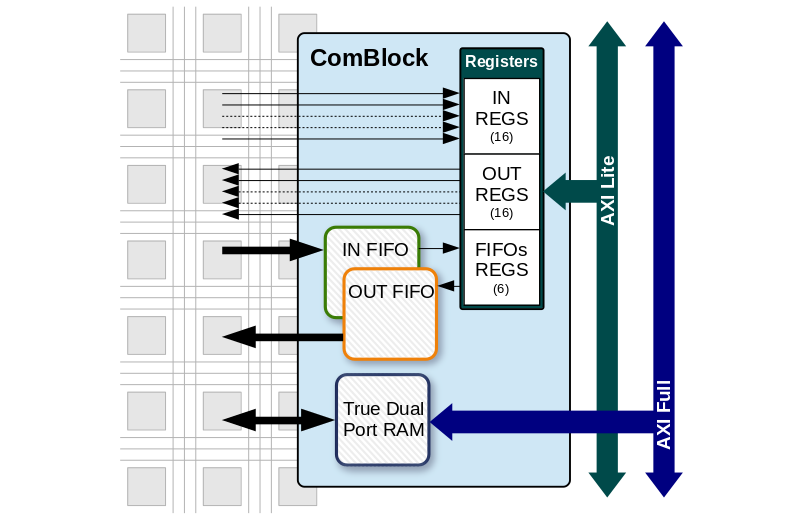
\includegraphics[width=12cm]{images/comblock.png}
    \end{center}
    \caption{Comblock schematic taken from \cite{FilesMasterRodrigo2021}}
    \label{fig:comblock_schematic}
\end{figure}

The integration of the ComBlock into a Vivado design follows a Plug-and-Play methodology within the IP Integrator environment. Once added to the Block Design, the ComBlock is connected to the Zynq Processing System through the AXI Interconnect, this task can be done automatically with the Vivado-IDE functions.

\begin{itemize}
    \item \textbf{Input and Output Registers:} Up to $32$ registers per direction for configuration parameters (e.g., enabling/resetting acquisition) and instantaneous status readout (e.g., cumulative fringe counts).
    \item \textbf{Asynchronous Input and Output FIFOs:} Buffered streaming channels built on internal Block RAM (\texttt{BRAM}) that safely transfer multi-bit event records or fringe timestamps across independent \texttt{PL}/\texttt{PS} clock domains.
    \item \textbf{True Dual-Port RAM (\texttt{TDPRAM}):} Shared memory accessible asynchronously by both the \texttt{PL} hardware and the \texttt{PS} processor.
\end{itemize}
By hiding the underlying AXI protocol complexity, the ComBlock enables the interferometer logic to connect directly via simple register and true dual RAM ports.


\subsection{PYNQ}

The development of custom hardware on FPGAs has traditionally been governed by Hardware Description Languages (HDLs), such as VHDL and Verilog. Unlike high-level programming languages (C or Python) that follow a sequential execution model, HDLs are used to describe the concurrent behavior and structural connectivity of digital logic. This fundamental difference imposes a steep learning curve on researchers, as hardware design requires deep knowledge of digital electronics and clock domain crossing. The productivity gap in FPGA design originates from the fact that even minor changes in a digital circuit require a full synthesis and implementation cycle, which can take from several minutes to hours. Furthermore, interfacing the hardware logic with a host computer for data analysis usually involves writing drivers in C. To address these challenges, the PYNQ framework was introduced \cite{PYNQ}.


The core innovation of PYNQ is the introduction of Hardware Overlays. An overlay is a pre-compiled, highly-optimized bitstream that acts as a hardware library. Just as importing a library into python to perform complex mathematical operations without knowing the underlying assembly or C code, a PYNQ user can load an overlay into the FPGA dynamically at runtime. By using overlays, the complexity of the HDL design is encapsulated into a functional block with a standardized interface (typically AXI-based for communication PL-PS). This allows the researcher to treat the FPGA as a high-performance co-processor that can be reconfigured through simple Python commands.


This approach simplifies FPGA usage in three key ways:
\begin{itemize}
\item \textbf{High-Level Interfacing:} Low-level memory-mapped I/O and DMA transactions are abstracted into Python objects. For instance, writing to an FPGA register becomes as simple as assigning a value to a variable in a Jupyter Notebook.
\item \textbf{Ecosystem Integration:} Because the data resides in a Python environment, it can be passed directly to scientific libraries such as \textit{NumPy}, \textit{Pandas}, and \textit{Matplotlib}. For numerical processing, for data management, and real-time visualization.
\item \textbf{Rapid Prototyping:} The use of Jupyter Notebooks allows for an interactive development workflow. Researchers can test hardware triggers, adjust acquisition parameters, and analyze data in a single, documented environment, significantly reducing development time.
\end{itemize}

\subsection{HDL on Git (Hog)}
The management of FPGA projects within traditional version control systems present significant challenges. Tools like AMD Vivado used for the design of the FPGA typically generate large binary project files that are not suited for line-by-line differencing. Furthermore, these tools frequently rely on absolute paths and local environment configurations, which severely hinders the ability to compile in a different machine without substantial changes to the codebase. This complicates the ability of multiple researchers to collaborate on a shared codebase without encountering conflicts. To overcome these limitations, the Hog(HDL on Git) framework \cite{HogHogGitLab2026} was developed, primarily at the European Organization for Nuclear Research (CERN), to provide a structured, Tcl-based methodology for handling HDL code within Git repositories. 

Tcl (Tool Command Language) is the standard language used to automate and control Electronic Design Automation (EDA) tools, such as AMD Vivado or Intel Quartus; These EDAs are built on a Tcl-first architecture. This means that every action you perform in the Graphical User Interface (GUI), such as clicking "Run Synthesis" is translated by the software into a specific Tcl command and executed in an internal console. This means that the construction of a project can be done with the appropriate use of Tcl commands.


Hog unifies the HDL development cycle by shifting the project definition from a GUI-centric model to a recipe-based model. In a Hog-managed repository, the Vivado project file is treated as a disposable, temporary artifact. The source to reconstruct the Vivado project resides in plain-text List Files (.src, .con, .sim; extensions created and managed by Hog), which contain relative paths to all source code, block design, constraints, and IP cores.

This approach reduces development time by allowing automated project creation. A new collaborator can recreate the entire local development environment including Block Designs, IP configurations, and synthesis settings by running a single script. This eliminates the manual setup phase that often leads to human error. Another great advantage of Hog is its direct integration to Git Submodules. This is particularly relevant for the integration of external IPs, such as the \textbf{ComBlock}, \cref{sec:comblock}, allowing different teams to maintain separate repositories for specific modules while integrating them into a top-level design. 

A critical feature of Hog regarding traceability is the automatic versioning system. During the synthesis process, Hog queries Git to retrieve the unique commit SHA and a hex-formatted timestamp. These values are automatically embedded into the firmware registers. This ensures that every bitstream generated is uniquely linked to a specific state of the source code, allowing researchers to know exactly which version of the logic is running on a detector at any given time.


Hog improves replicability, it ensures that any researcher can clone an open-hardware repository, like the one presented in \cref{sec:comblock_API}, and produce a bitstream that is functionally identical. 


\subsection{Comblock API for PYNQ} 
\label{sec:comblock_API}
% \label{sec:comblock_pynq_api}

\begin{figure}[htbp]
\centering
\resizebox{\textwidth}{!}{%
\begin{tikzpicture}[
    >=Latex,
    font=\small,
    layer/.style={draw, rounded corners=5pt, align=center, inner sep=6pt},
    card/.style={draw, rounded corners=4pt, align=center, inner sep=5pt, fill=white},
]

    % =========================================================
    % Layer 1: User Application (PYNQ / Jupyter)
    % =========================================================
    \node[layer, fill=blue!8, draw=blue!65!black, thick,
          minimum width=14.2cm, minimum height=1.2cm] (user_app) at (7.5, 10.7) {
        \textbf{\color{blue!65!black}User Application Layer (PYNQ / Jupyter Notebook)}\\[3pt]
        \footnotesize High-level Python control \& NumPy data analysis (no raw memory addresses)
    };

    % =========================================================
    % Layer 2: Comblock_API_for_PYNQ Abstraction Layer
    % =========================================================
    \draw[layer, fill=teal!6, draw=teal!70!black, very thick]
        (0.4, 6.2) rectangle (14.6, 9.2);
    \node[font=\small\bfseries, text=teal!70!black] at (7.5, 8.82)
        {\texttt{Comblock\_API\_for\_PYNQ} (Driver Abstraction Layer)};

    \node[card, draw=teal!65!black, thick,
          minimum width=4.3cm, minimum height=1.8cm] (card_reg) at (2.6, 7.45) {
        \textbf{Registers}\\[3pt]
        \footnotesize Control \& status\\
        \footnotesize \textit{(bounds \& R/W safe)}
    };

    \node[card, draw=teal!65!black, thick,
          minimum width=4.3cm, minimum height=1.8cm] (card_fifo) at (7.5, 7.45) {
        \textbf{FIFOs}\\[3pt]
        \footnotesize Buffered streaming\\
        \footnotesize \textit{(status \& bulk NumPy I/O)}
    };

    \node[card, draw=teal!65!black, thick,
          minimum width=4.3cm, minimum height=1.8cm] (card_dram) at (12.4, 7.45) {
        \textbf{DRAM}\\[3pt]
        \footnotesize Shared block memory\\
        \footnotesize \textit{(fast NumPy slicing)}
    };

    % =========================================================
    % Layer 3: PYNQ MMIO & AXI4 Buses (PS <-> PL)
    % =========================================================
    \node[layer, fill=orange!10, draw=orange!75!black, thick,
          minimum width=9.2cm, minimum height=1.15cm] (bus_lite) at (5.05, 4.65) {
        \textbf{\color{orange!75!black}PYNQ \texttt{MMIO} \& AXI4-Lite Bus}\\[2pt]
        \footnotesize 32-bit register \& FIFO transfers (PS $\leftrightarrow$ PL)
    };

    \node[layer, fill=orange!10, draw=orange!75!black, thick,
          minimum width=4.3cm, minimum height=1.15cm] (bus_full) at (12.4, 4.65) {
        \textbf{\color{orange!75!black}AXI4-Full Bus}\\[2pt]
        \footnotesize Burst memory transfers
    };

    % =========================================================
    % Layer 4: ICTP ComBlock IP Core (PL)
    % =========================================================
    \draw[layer, fill=violet!8, draw=violet!70!black, thick]
        (0.4, 1.85) rectangle (14.6, 3.35);
    \node[font=\small\bfseries, text=violet!70!black] at (7.5, 3.0)
        {ICTP ComBlock IP Core (Programmable Logic)};

    \node[card, draw=violet!50, minimum width=4.3cm, minimum height=0.72cm]
        at (2.6, 2.32) {\footnotesize Async I/O Registers};
    \node[card, draw=violet!50, minimum width=4.3cm, minimum height=0.72cm]
        at (7.5, 2.32) {\footnotesize Async BRAM FIFOs};
    \node[card, draw=violet!50, minimum width=4.3cm, minimum height=0.72cm]
        at (12.4, 2.32) {\footnotesize Dual-Port RAM};

    % =========================================================
    % Layer 5: Custom Interferometer Gateware (Arty Z7-20 PL)
    % =========================================================
    \node[layer, fill=gray!12, draw=gray!70!black, thick,
          minimum width=14.2cm, minimum height=1.15cm] (pl_logic) at (7.5, 0.55) {
        \textbf{Interferometer Acquisition Logic (Arty Z7-20 PL)}\\[3pt]
        \footnotesize Photodiode Digital Input $\rightarrow$ Synchronizer \& Edge Counter $\rightarrow$ Fringe Data
    };

    % =========================================================
    % Clean Vertical Arrows Between Layers
    % =========================================================
    % Layer 1 <-> Layer 2
    \draw[<->, thick, blue!60!black] (2.6, 9.2) -- (2.6, 10.1);
    \draw[<->, thick, blue!60!black] (7.5, 9.2) -- (7.5, 10.1);
    \draw[<->, thick, blue!60!black] (12.4, 9.2) -- (12.4, 10.1);

    % Layer 2 <-> Layer 3
    \draw[<->, thick, teal!70!black] (2.6, 5.23) -- (2.6, 6.2);
    \draw[<->, thick, teal!70!black] (7.5, 5.23) -- (7.5, 6.2);
    \draw[<->, thick, teal!70!black] (12.4, 5.23) -- (12.4, 6.2);

    % Layer 3 <-> Layer 4
    \draw[<->, thick, orange!75!black] (2.6, 3.35) -- (2.6, 4.07);
    \draw[<->, thick, orange!75!black] (7.5, 3.35) -- (7.5, 4.07);
    \draw[<->, thick, orange!75!black] (12.4, 3.35) -- (12.4, 4.07);

    % Layer 4 <-> Layer 5
    \draw[<->, thick, violet!70!black] (2.6, 1.13) -- (2.6, 1.85);
    \draw[<->, thick, violet!70!black] (7.5, 1.13) -- (7.5, 1.85);
    \draw[<->, thick, violet!70!black] (12.4, 1.13) -- (12.4, 1.85);

\end{tikzpicture}%
}
\caption{High-level layered architecture of Comblock API for PYNQ \cite{gallegoJcgallego1Comblock_API_for_PYNQ2026}, bridging Python analysis scripts to the interferometer PL gateware via safe register, FIFO, and DRAM abstractions.}
\label{fig:comblock_api_arch}
\end{figure}


Although the ICTP ComBlock eliminates custom AXI finite-state machines on the Programmable Logic (PL) side, interacting with it directly from the Zynq Processing System (PS) using raw memory-mapped I/O (MMIO) still exposes low-level hardware details to the user. Without an abstraction driver, Python scripts must calculate byte-aligned hexadecimal register offsets manually, perform bitwise masking and shifting to interpret FIFO status flags, and enforce array bounds by hand—increasing the risk of silent data corruption, FIFO overflows/underflows, or accidental writes to read-only hardware registers.

To eliminate these low-level error modes and bridge the ComBlock cleanly into the PYNQ ecosystem, a dedicated object-oriented Python driver (Comblock API for PYNQ) was implemented \cite[Repository]{gallegoJcgallego1Comblock_API_for_PYNQ2026}. Built on top of PYNQ's DefaultIP class, the Comblock driver inspects the Vivado hardware handoff (\emph{.hwh}) metadata when an overlay is loaded and automatically binds to the IP core instance (e.g., \emph{cb = overlay.comblock\_0}). Rather than exposing flat memory addresses, it organizes the hardware into three specialized sub-interfaces:

\begin{itemize}
    \item \textbf{Register Interface (\emph{IN\_REGS}, \emph{OUT\_REGS}):} Provides boundary-checked \emph{read(offset)} and \emph{write(offset, value)} operations for 32-bit AXI4-Lite registers. Out-of-bounds indices raise \emph{IndexError}, while write attempts to read-only input registers raise \emph{PermissionError}, preventing invalid bus accesses.
    \item \textbf{Fifo Interface (\emph{FIFO\_IN}, \emph{FIFO\_OUT}):} Decodes raw hardware status bitmasks via \emph{get\_status()} into a readable Python dictionary (\emph{occupancy}, \emph{empty}, \emph{full}, \emph{almost\_empty}, \emph{almost\_full}, \emph{underflow}, and \emph{overflow}). High-throughput \emph{read\_bulk()} and \emph{write\_bulk()} methods transfer blocks directly to and from NumPy arrays while guarding against buffer overflows/underflows (\emph{RuntimeError}), and \emph{reset()} safely flushes pending entries.
    \item \textbf{Dram Interface:} Exposes AXI4-Full shared memory through vectorized
    \emph{read\_bulk}\allowbreak\emph{(offset,\allowbreak count)} and
    \emph{write\_bulk}\allowbreak\emph{(offset,\allowbreak data)} calls backed by NumPy slicing for fast block transfers.
\end{itemize}

\paragraph{Significance for the Interferometer Acquisition System.}
Introducing Comblock API for PYNQ provides three decisive advantages for experimental operation (\cref{fig:comblock_api_arch}):
\begin{enumerate}
    \item \textbf{Hardware-Safe Experimentation:} Automatic bounds, permission, and FIFO-occupancy checks prevent illegal hardware states during interactive Jupyter Notebook sessions, allowing rapid reconfiguration of gating, resets, and readout intervals without crashing the AXI bus.
    \item \textbf{Direct Scientific Computing Integration:} By returning NumPy arrays directly from \emph{FIFO\_IN.read\_bulk()} and \emph{DRAM.read\_bulk()}, captured fringe counts and nanosecond timestamps feed seamlessly into Python analysis routines (velocity reconstruction, spectral analysis, and visualization) without slow per-sample Python loops.
    \item \textbf{Decoupled Software–Gateware Maintenance:} Application scripts reference semantic methods (such as \emph{cb.IN\_REGS.read(0)}) rather than hardcoded hexadecimal addresses, keeping host software portable across different Zynq boards.
\end{enumerate}


